\documentclass[a4paper,11pt]{article}
\usepackage[T1]{fontenc}
\usepackage[utf8]{inputenc}
\usepackage{lmodern}
\usepackage{hyperref}
\usepackage{graphicx}
\usepackage{rotating}
\usepackage{listings}
\usepackage{color}
\usepackage{appendix}
\usepackage{caption}
\usepackage{float}

% Swedish
\usepackage[swedish]{babel}

% Table of contents depth 3 levels: A.B.C
\setcounter{tocdepth}{3}

\begin{document}

\title{{\huge Sommarstugekoll} \\
	Digital Konstruktion EDA234 \\ Grupp 2}
\author{Fredrik Brosser, Karl Buchka, Andreas Henriksson, Johan Wolgers \\ \\
   	Chalmers Tekniska Högskola \\ \\
	\begin{tabular}{l c r}
		\texttt{frebro} & \texttt{@} & \texttt{student.chalmers.se}\\
		\texttt{karlbu} & \texttt{@} & \texttt{student.chalmers.se}\\
		\texttt{henriksa} & \texttt{@} & \texttt{student.chalmers.se}\\
		\texttt{wolgers} & \texttt{@} & \texttt{student.chalmers.se}\\\\
	\end{tabular}
	}

\maketitle
 \thispagestyle{empty}
\pagebreak
 \thispagestyle{empty}
	\tableofcontents
 \thispagestyle{empty}

\pagebreak


\begin{center}
	{\noindent \bf Sammanfattning}
\end{center}

	Ett system för temperaturavläsning och relästyrning beskrivs genom denna rapport. Systemet är åtkomligt och styrbart via telefon genom DTMF (Dual Tone Multiple Frequency). Systemets funktion består i att informera användaren om aktuella temperaturer från två temperatursensorer samt ge användaren möjlighet att via telefon styra utgångarna (till/från) för exempelvis värmeelement eller belysning. Styrning och återkoppling utbytes genom en telefonlinje, POTS (Plain Old Telephone Service) med hjälp av DTMF.

En tänkt tillämpning för produkten:
\begin{list}{*}{}
\item Systemet inkopplas innan avfärd från sommarstugan och befinner sig i viloläge. 
\item Användaren kan då denne önskar ringa upp systemet som på anmodan returnerar temperatur från någon av temperaturgivarna.
\item Användaren kan sedan genom sin knapptelefon aktivera eller avaktivera någon av utgångarna för att på så sätt slå till värme, belysning eller vad som anslutits till funktionsutgångarna.
\end{list}

\begin{center}
	{\noindent \bf Abstract}
\end{center}

	The system described in this report is an automated domestic temperature control system, accessible and controllable via
	a standard telephone connection (DTMF). The main functionality of the system is informing the user of the current temperatures
	at the points of measurement, and also to give the user the ability to remotely control (simple on/off) a number of external
	functions. These functions could be, for example, heating systems, radiators or air conditioning. Information- and control data
	is exchanged via a standard, analog telephone connection, using DTMF: Dual Tone, Multiple Frequency.

	A specific, practical usage example is the concerned holiday home owner wanting to keep control of the heating in his summer house.
	Using Sommarstugekoll, one can keep the temperature at a reasonable level, avoiding for example pipes freezing, but at the same time
	keeping the total heating costs to a minimum. Sommarstugekoll solves this by offering users a neat and simple way to keep track
	of in- and outdoor temperatures - when the previously mentioned summer house owner wishes to make a visit, he simply dials the
	summer house telephone number giving it instructions to bring the temperature up to a comfortable level, all while he makes
	the drive up. Simple - smart - elegant - Sommarstugekoll is the domestic temperature automation assistant of the future!
 \thispagestyle{empty}
\pagebreak

\setcounter{page}{1}
\section{Introduktion}

	Konstruktionsprojektet utförs inom kursen ``Digital Konstruktion, EDA234'' vid Chalmers Tekniska Högskola. Uppgiften består att inom gruppen om 4 personer konstruera och dokumentera
	ett digitalsystem utifrån en specifikation, med fokus låg på huvudfunktionalitet i det digitala området. Utvecklingen sker på ett färdigt utvecklingskort vilket sedan kompletteras med externa kretsar och programmeras för att nå kravspecefikationen. Logikkretsen som används är en Xilinx XC9572XL CPLD, och utveckligen sker i huvudsak med VHDL i Xilinx ISE-miljön samt i ModelSim för simuleringar. Rapporten är uppdelad i abstraktionslager med fördjupningar i de senare avsnitten. 

	En handhavandeinstruktion återfinns bifogad i Appendix~\ref{sec:Manual}.

\pagebreak

\section{Kravspecifikation och systembeskrivning}
	Systemet består av en styrenhet placerad på två CPLD med anslutning till telefonnätet. Sytrenheten har med hjälp av en DTMF avkodare möjlighet att tolka användarens telefonknapptryckningar på distans. Vidare kan användaren genom dessa knapptryckningar skicka signal för att hämta datavärde från någon av de två temperaturgivarna, anslutna anslutns med entrådsbus, en röstenhet läser sedan upp ett förinspelat meddelande för respektive temperatur. Vidare kan användaren också starta eller stoppa någon av de funktionsutgångar som finns till hands, användaren får då akustisk återkoppling om aktuell status för funktionsutgången via samma ljudmodul.

Funktionsutgångarna kan också styras lokalt med med bifogade knappsatsen. Aktuell status för funktionsutgångarna visas med lysdioder. 

	\subsection{Tolkning och definition av kravspecifikation}

		Inom det tilltänkta användningsområdet, ett fritidshus med POTS-linje som under större delen av året endast nyttjas tillfälligtvis, är det rimligt med en temperatur om $5-10\,^{\circ}\mathrm{C}$ då ingen vistas i huset. Vidare bör det vara önskvärt att ha möjlighet att slå till normal värme innan ett besök, kunna kontrollera att det blivit varmt samt att kontrollera att temperaturen är över $0\,^{\circ}\mathrm{C}$. Systemet kan därför tolka en temperatur om $\pm 32\,^{\circ}\mathrm{C}$ från givarna med en upplösning om $\pm 1\,^{\circ}\mathrm{C}$. Senast avläst temperatur visas också binärt på LED-displayen.

		Systemet matas med en spänning om $5\,V$ DC, då systemet är till indikeras detta med en lysdiod.

	\subsection{Uppdelning}

	Systemet är uppdelat i ett antal delblock (moduler) och är konstruerat för att vara så modulärt som möjligt.
	Nedan följer en sammanfattande tabell över hur de olika modulerna är uppdelade på de två CPLD:erna. Varje modul är mer
	utförligt beskriven i respektive sektion under rubriken ~\ref{sec:Funktionsenheter} \nameref{sec:Funktionsenheter}. 

	I blockschema som återfinns i figur~\ref{fig:blocks1} och~\ref{fig:blocks2} visas respektive modul och uppdelningen på två CPLD samt dess kommunikationsvägar. I tabell~\ref{tab:uppdelningstabell} förklaras respektive modul samt vilken CPLD som innehåller denna.\\\\

	\begin{figure} [H]
		  	
			\centering
			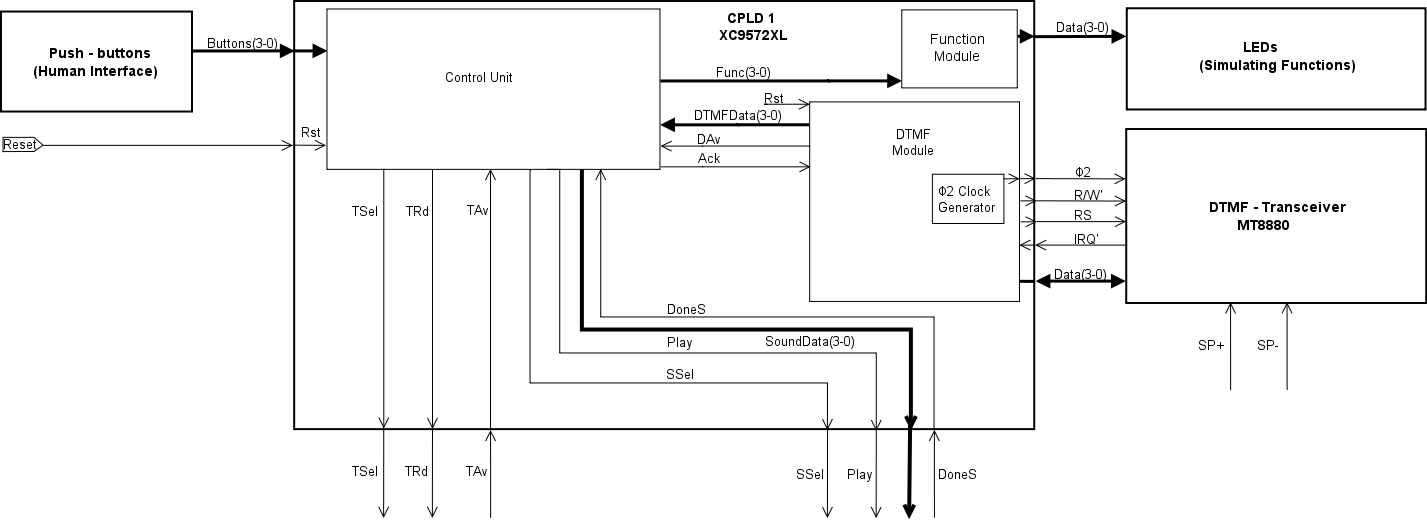
\includegraphics[width=1\textwidth]{BlockDiagramCPLD1.png}
		  	\caption{Blockdiagram för CPLD1}
			\label{fig:blocks1}
	\end{figure}

	\begin{figure}[H]
		  	
			\centering
			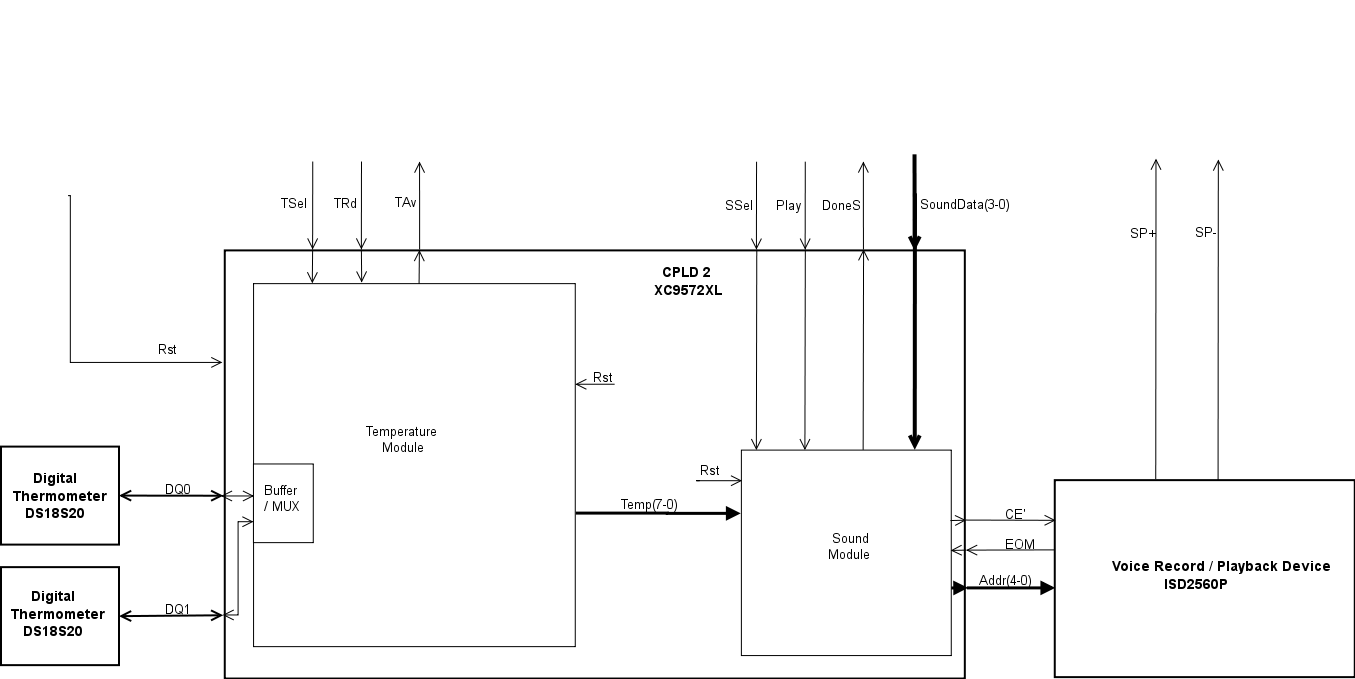
\includegraphics[width=1\textwidth]{BlockDiagramCPLD2.png}
			\caption{Blockdiagram för CPLD2}
			\label{fig:blocks2}
	\end{figure}

	\begin{table} [H]
		
		\caption{Respektive CPLD's moduler och uppgifter} 
		\label{tab:uppdelningstabell}
	\begin{tabular}{l l}
		
		{\bf CPLD1} \\
		Modul	& Funktion	\\
		\hline
		Styrenhet	& Samordnar systemets funktion \\
		DTMF-modul & Tar emot DTMF-signaler via POTS \\
		Funktionsmodul	& Hanterar funktionsutgångarna \\
		Knappmodul	& Hanterar tryckningar på knappsatsen \\
		\\
		{\bf CPLD2} \\
		Modul	& Funktion	\\
		\hline
		Temperaturmodul	& Initierar, läser och presenterar temperatur \\
		Ljudmodul	& Hanterar styrning av extern ljudmodul \\
		
	\end{tabular}
	\end{table}
	
	Systemet är uppdelat enligt ``dataväg-styrenhet-modellen'', där designprincipen går ut på att skilja styrsignaler
	och dataflödeskontroll (Styrenheten) från datan som forslas genom systemet (Datavägen). Systemet skickar temperaturdata från temperaturmodulen till ljudmodulen samt adressdata till ljludlagringsenheten från ljudmodulen. Detta flöde kontrolleras från styrenheten via
	enkla styrsignaler. Viss data, i form av indata från användargränssnitt och styrsignaler till funktionsutgångar, passerar dock genom styrenheten.

	\subsection{Arbetsflöde}

I sitt viloläge väntar systemet på inkommande samtal. Då samtal mottages börjar systemet börjar med att läsa upp ett antal ljudklipp med aktuella temperaturer, och erbjuder sedan användaren möjligheten till att styra de externa funktionerna. Telefonen skickar ut DTMF-signaler, som läses och avkodas av DTMF-transceivern, MT8880, vilken avkodar tvåtonssignalerna för att unikt identifierna nedtryckt knapp och sänder ut denna på databussen till DTMF-modulen. 

Då användaren nedtrycker en knapp sker följande. Motsvarar knapptryckningen ett funktionskommando (funktion till eller från) så sätter CPLD'n statusen för respektive funktionsutgång. \colorbox{yellow}{Lägg eventuellt in andra knapptryckningar som kan motsvara kommandon här}

\section{Funktionsenheter}
\label{sec:Funktionsenheter}
Systemet är som tidigare nämnt uppdelat i sex funktionsenheter vilka nedan presenteras närmare.

	\subsection{Dataväg}
	Temperaturdatan avläses från temperatursensorer och skickas till temperaturmodulen denna skickar sedan datan vidare till ljudmodulen, för vidare uppläsning via ljudlagringskretsen, ISD2560P. Denna data skickas aldrig genom, men kontrolleras av, styrenheten. Den rena datavägen i systemet är alltså här begränsad till CPLD2.
	
	\subsection{Styrenhet}

	Styrenheten kontrollerar och ger styrsignaler för att hantera de övriga systemdelarna. Syftet är att ge en lätt överblick över hela körcykeln, där styrenheten har kontroll över funktionerna via en rad styr-, available- och acknowledgesignaler. Styrenheten får även indata från knappsats och DTMF-mottagare via respektive modul som presenterar data för styrenheten. Denna indata är skild från datavägen (temperaturinformation), och meddelar styrenheten om näsföljande steg, dvs. reagera i enlighet med användarsignaler.

	\subsubsection{Uppbyggnad}

	Styrenheten är i sin tur modulärt uppbyggd, och har ett väl avgränsat interface mot varje annan delmodul, men fungerar samtidigt som en samordnare mellan de olika modulerna.	För en ingående grafisk beskrivning av den bakomliggande tillståndsmaskinen, se sektion~\ref{sec:Tillstandsmaskiner} ~\nameref{sec:Tillstandsmaskiner}.

	\subsection{DTMF-Modul}
		
	DTMF-modulen i CPLD1 är ansvarig för att hantera kommunikation med telefonen och därmed också med användaren.
	När användaren trycker ner en knapp på telefonen genereras en DTMF-signal som uppfattas och avkodas av DTMF-modulen vilken sedan presenterar den mottagna indatan för styrenheten.
		
	\subsubsection{Initiering}

	DTMF-modulen måste få en initieringspuls minst 100 ms efter spänningspåslag. Detta sker med hjälp av
	en extern tryckknapp, som beskrivet i användarmanualen. Under hela initieringen är Chip Select satt låg
	och RS0 satt hög. Initieringscykeln börjar med att DTMF-modulen läser statusregistret och ger kommandon genom att skriva till kontrollregistret på MT8880-kretsen enligt ett i databladet givet mönster, se även sektion ~\ref{MT8880C} under~\nameref{hårdvara} för vidare beskrivning.
	DTMF-Modulen är ansvarig för att ge ut rätt signaler under initieringsfasen, vilket görs med hjälp av en tillståndsmaskin vilken finns vidare beskriven i sektion~\ref{sec:Tillstandsmaskiner} ~\nameref{sec:Tillstandsmaskiner}.
		
	\subsubsection{Läsning}

	Då initieringen av MT8880C är färdigställd går DTMF-Modulen över i ett läsläge, där den kontinuerligt lyssnar efter insignaler från MT8880C-kretsen. När giltig indata detekteras läses den och läggs ut på den interna DTMF-databussen till styrenheten, varpå DTMF-Modulen ger signal  ``dAv'' till styrenheten. DTMF-modulen väntar sedan på en bekräftelsesignal (dAck) från styrenheten. Läsningen sker genom att DTMF-modulen väntar på signal på avbrottsutgången (IRQ) vilket betyder att en ny DTMF-signal detekterats  och avkodats från telefonlinjen och lagts ut på databussen från MT8880C'n.


	\subsection{Ljudmodul}

		\subsubsection{Modulbeskrivning}

		\subsubsection{Initiering}

		\subsubsection{Addressering och Uppspelning}

	\subsection{Temperaturmodul}

	Temperaturmodulen är ansvarig för att hantera seriekommunikationen med 
	DS18S20-temperatursensorerna, via entrådsbussarna, samt att ge ut de lästa temperaturerna
	i tecken-belopp-format, där den mest signifikanta biten ger tecknet (positiv eller negativ) och efterföljande bitar temperaturdatan binärt.
	Temperaturerna skickas via en intern databuss till ljudmodulen, i syfte att låta den i sin tur spela upp de avlästa temperaturen för användaren. 
	För vidare beskrivning av temperatursensorkretsen, se sektion ~\ref{DS18S20} under~\nameref{hårdvara}.

	\subsubsection{Entrådsbuss}

	Temperaturmodulen kommunicerar seriellt med temperatursensorn över en entrådsbuss.
	Entrådsbussen är ansluten till matningsspänning (+5V) genom ett pull-up-motstånd på 4.7kOhm, och
	ändarna av bussen är anslutna till mastern (CPLD) och sensorn (DS18S20), respektive. Då bussen
	befinner sig i viloläge dras den hög ("svag drivning") av pull-up-motståndet. När information
	skickas över bussen drar den kommunicerande (sändande) enheten bussen låg genom att driva den
	med en stark logisk nolla.

	\subsubsection{Läscykel}

	En läscykel består av fyra steg: initialisering, kommandon, läsning och viloläge.

	(Se även figur ~\ref{fig:RCFlowChart} för en flödesdiagram-beskrivning av en hel läscykel.)

	Initialiseringen består i av att mastern driver bussen låg i 512 us, sedan släpper den.
	Temperatursensorn svarar då med en närvaro-puls genom att driva bussen låg i 106 us.

	Då mastern detekterat närvaropulsen börjar den överföra ett ROM-kommando (Skip ROM, 0xCC), följt av en kort återhämtningslucka och sedan ett Funktions-kommando (Convert Temperature, 0x44), enligt läs-/skriv-luckemetoden som beskrivits ovan.
	Skip-ROM-kommandot används i det här systemet eftersom endast en temperatursensor används per entrådsbuss.
	Därmed finns inget behov av att kunna addressera specifika sensorer på bussen.
	Då Convert Temperature-kommandot ges gör DS18S20-kretsen en temperaturkonvertering, för att sedan spara den lästa temperaturdatan i ett internt 9-bytes minne.
	Under konverteringsperioden (upp till 750 ms) kan mastern göra polling av temperatursensorns status. Detta innebär att mastern kontinuerligt
	sänder förfrågningar genom att dra bussen låg i en kort period (4 us). Temperatursensorn svarar med en nolla
	då konvertering sker, och en etta då konverteringen är klar.
	Då mastern ser att konverteringen är klar, initialiseras temperatursensorn om och ytterligare ett ROM-Funktions-kommandopar överförs. Dessa är 0xCC (Skip ROM) följt av 0xBE (Read Scratchpad), respektive.
	Idealt ska temperatursensorkretsen nu vara redo att överföra temperaturdata till mastern från sitt interna 9-bytesminne.
	Då den ges Read Scratchpad-kommandot börjar DS18S20 sända över innehållet i sitt minne över bussen.
	Mastern går då in i läsningsläget och börjar sampla datan på bussen genom att driva bussen låg, släppa den och sampla efter 4 us.
	Mastern samplar de första åtta bitarna data som sänds av DS18S20, sedan en ytterligare, nionde bit. 
	Den sista biten utgör en tecken-bit för att avgöra om temperaturen är positiv eller negativ. Då den nionde biten data lästs
	ger mastern på nytt en initieringspuls, som säger åt temperatursensorn att sluta sända data.
	Den nyligen lästa temperaturen placeras på den interna temperaturbussen, och temperaturmodulen signallerar till styrenheten att giltig data finns på bussen.

		\begin{figure}[ht!tb]
		  \centering
		      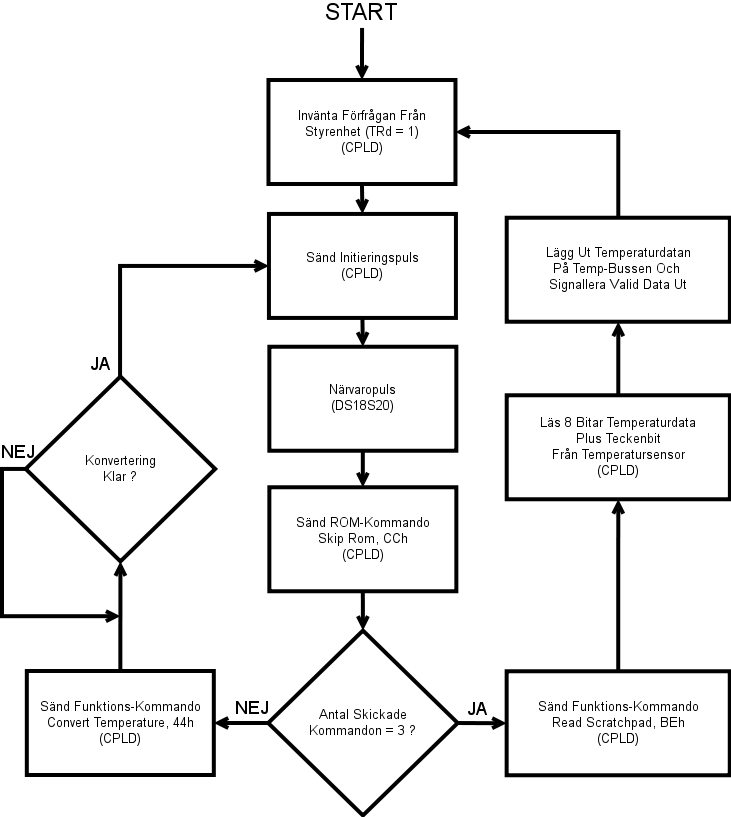
\includegraphics[scale=0.5, angle=0]{ReadCycleFlowChart.png}
		  	\caption{Högnivå-flödesdiagram för Temperaturläscykel}
			\label{fig:RCFlowChart}
		\end{figure}

	\subsubsection{Uppbyggnad}

	Temperaturmodulen är baserad runt en tillståndsmaskin, understödd av en intern Buffer/MUX-modul samt 
	ett antal interna räknare för att generera de nödvändiga tidsfördröjningspulserna. För en grafisk beskrivning av den interna tillståndsmaskinen som används av temperaturmodulen,
	se sektion~\ref{sec:Tillstandsmaskiner} ~\nameref{sec:Tillstandsmaskiner}.

	\subsubsection{Buffer/MUX}

	Buffern är en tri-state-buffer med en Enable-signal.
	Buffer/MUX-modulen är direkt ansluten till de två DS18S20-Temperatursensorerna som använder entrådsbusskommunikationen.
	Multiplexern (MUX) används för att välja mellan vilken av de två sensorerna som styrenheten vill kommunicera med.

	\subsubsection{Räknare}

	Internt använder temperaturmodulen ett antal olika räknare: \\
		\begin{tabular}{l c r}
			\\{\bf Namn} & {\bf Bitar} & {\bf Beskrivning}\\
			cntInt & 9 & Genererar timing-pulser\\
			ZC & 4 & Hanterar timing för skriv-luckor\\
			Progress & 2 & Anger aktuellt kommando (0-3)\\
			bitCnt & 8 & Anger aktuell bit för överföring/läsning\\\\
		\end{tabular}

	Se sektion~\ref{sec:programlistningar} ~\nameref{sec:Programlistningar}.

	\subsection{Extern funktionsstyrning}

Funktionsmodulen är mycket enkelt uppbyggd, den tar emot data från Styrenheten och skickar vidare 
uppdateringarna ut på de I/O-pinnar som används för funktionerna. Sammanfattat fungerar den som ett
mellansteg för att underlätta för styrenhetens funktionsstyrning, och kan vid behov byggas ut ytterligare
för att implementera andra funktioner i systemet.

	\subsection{Användargränssnittshantering}

Systemet har, förutom DTMF-kontroll, även ett fysiskt gränssnitt med en knappsats samt en till/från-brytare för temperaturläsning.
Dessa rådata måste formateras, avkodas och presenteras för styrenheten. Detta är knappsatsmodulens uppgift.

Om en knapp på knappsatsen trycks ned, skickas en availablesignal (DAv) från knappsatsen till knappsatsmodulen, som sedan
avkodar vilken knapp som tryckts ned, och presenterar detta för styrenheten genom att höja en KAv (Keyboard Available)-signal,
vilket indikerar valid data på knappsatsdatabussen, KData[3..0]. Genom att skicka en Acknowledgement-signal, KAck, bekräftar 
styrenheten att den sett och mottagit datan från knappsatsen.

\section{Hårdvara}
\label{hårdvara}
	\subsection{ISD2560P}

	\subsection{DS18S20}
	\label{DS18S20}
		Den temperatursensor som används är Maxim DS18S20, som ger temperaturmodulen möjlighet att läsa av temperaturen
		med nio (9) bitars upplösning. Sensorerna som användas i detta system drivs av en extern spänningskälla på +5V,
		och kommunicerar seriellt över en entrådsbuss. Seriekommunikationen baserar på att bus-mastern initierar skriv-
		och läs-luckor. Varje sådan lucka är mellan 60 och 120 us lång. Temperatursensorn initieras genom att mastern
		driver bussen låg i åtminstone 480 us, vilket följs av att temperatursensorkretsen själv drar bussen låg i 60-240 us,
		efter en återhämtningslucka på minst 1 us. Efter initieringen väntar sensorkretsen på ett ROM-kommando från mastern,
		följt av ett Funktions-kommando. Varje sådant kommando är en byte lång, och skickas som LSB-först. Mastern skickar
		en logisk nolla genom att driva bussen låg under hela skrivluckan. En etta skickas genom att mastern driver bussen låg
		under en kort period, 1-15us, och sedan släpper bussen under resten av skrivluckans längd. Mellan varje skriv- eller läslucka
		måste det finnas en återhämtningsperiod på minst 1us.

		Då mastern är klar med att skicka över ROM- och Funktions-kommando, kan (beroende på vilka kommandon som sändes) DS18S20-kretsen
		svara med aktuell data. På samma sätt som ovan måste mastern här initiera en läs-lucka genom att driva bussen låg i 1-8us, och
		sedan släppa den (högimpediv). DS18S20-kretsen svarar på den allokerade läs-luckan genom att antingen hålla bussen låg för att
		överföra en nolla, eller genom att låta bussen dras hög av pull-up-motståndet för en etta. Under den här tiden (upp till 15 us
		efter att ha släppt bussen) kan mastern sampla bussen för att läsa av vad DS18S20-kretsen skickat. All data som skickas från
		temperatursensorn skickas som LSB-först, och i 2-komplementsform.\\

	\subsection{MT8880C}
	\label{MT8880C}
		Avkodning av uppringandes DTMF-signaler avkodas med hjälp av MT8880C från Mittel. 
		Telefonsignalen kopplas direkt in till DTMF-överföraren enligt specifikation för standarsuppkoppling i datablad. Endast avkodningsfunktionen på 		kretsen används. Databuss, R/W-signal, IRQ och $\Phi$2 är anslutna till kontrollenheten. 
		CS (Chip Select) är satt konstant låg då denna krets använder bussen exklusivt. 
Före initiering skickas manuellt en initieringspuls till kretsen minst 100ms efter spänningspåslag. Detaljer om initieringscykeln finns i databladet för MT8880C.
\colorbox{yellow}{Referens till Datablad?} \\

\section{Tillståndsmaskiner}
\label{sec:Tillstandsmaskiner}		
\subsection{Styrenhet}
		\subsection{Temperaturmodul}
			Se state-machine-diagram: ~\ref{fig:TempSM} och förklaring ~\ref{fig:SMExp}\\
			{\bf Reset:} Alla signaler och räknare återställs till sina grundvärden.\\
			{\bf Grundvärden:} Utgångspunkten är att alla signaler behåller sina gamla värden om inget annat anges.\\
			\begin{tabular}{l}
				\\{\bf Viloläge (Tillstånd 0):}\\
				0: Viloläge och återställningspunkt. Inväntar TRd = 1 från Styrenheten\\
				{\bf Initialisering (Tillstånd 1-3):}\\
				1: Fördröjningstillstånd, väntar på puls på DelayLong (512 us)\\
				2: Mastern driver bussen låg i 512 us och sätter datavärdet till 0xCC (Skip ROM)\\
				3: Mastern släpper bussen, DS18S20 skickar närvaropuls\\
				{\bf Kommandoöverföring (Tillstånd 4-8):}\\
				4: Förberedelsetillstånd före sändning\\
				5: Huvudsändningstillståndet, mastern sänder bit enligt aktuellt räknarvärde\\
				6: Mellanbittillstånd, återhämtningstillständ. Fortsätter om fler bitar ska skickas\\
				7: Avgör om DS18S20 är upptagen med att konvertera temperaturen. Om så, vänta tills klar\\
				8: Vägskälstillstånd. Om vi har fler kommandon att skicka, gå tillbaka, annars börja läsa\\
				{\bf Läsning (Tillstånd 9-15):}\\
				9:  Förberedelsetillstånd före läsning\\
				10: Mastern initierar en läslucka genom att dra bussen låg i 4 us\\
				11: Mastern väntar ytterligare 4 us för att pull-up-motståndet ska få verka\\
				12: Mastern samplar bussen. Om DS18S20 skickar en nolla hålls bussen låg, annars inte\\
				13: Återhämtningstillstånd mellan samplingar\\
				14: Vägskälstillstånd. Om vi har fler bitar att läsa, gå tillbaka, annars gå vidare\\
				15: Läsning klar, lägg ut temperatur på buss och signallera valid data. Gå tillbaka till 0\\
			\end{tabular}

	\begin{figure}[ht!tb]
	  \centering
	      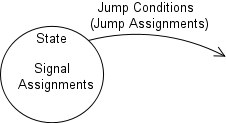
\includegraphics[scale=0.5, angle=0]{StateMachineExplained.png}
		\label{fig:SMExp}
	  	\caption{Förklaring till State Machine-diagram}
	\end{figure}

	\begin{figure}[ht!tb]
	  \centering
	      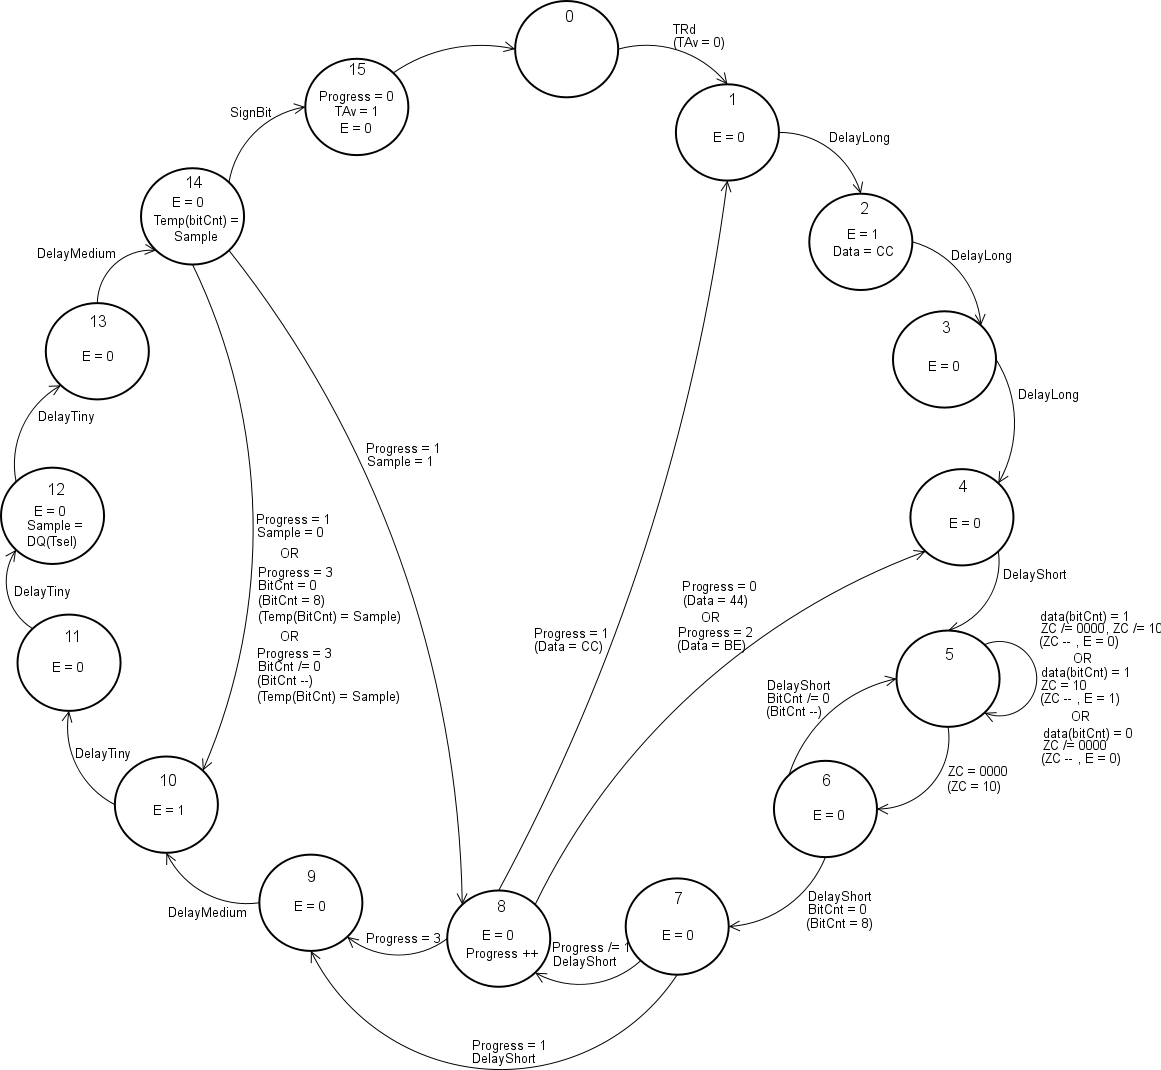
\includegraphics[scale=0.4, angle=0]{TempStateMachineDiagram.png}
		\label{fig:TempSM}
	  	\caption{Detaljerat State Machine-diagram för Temperaturläscykel}
	\end{figure}

		\subsection{DTMF-Modul}
		\subsection{Ljudmodul}

\section{Felanalys}

Då systemet hanterar avläsning av temperaturer och endast klarar ett begränsat temperaturintevall
görs här en felanalys. För de tillämpningsområden systemet är konstruerat för (hemanvändare) 
är mätfelen dock för små för att ha betydelse.

Temperatursensorerna arbetar med en temperaturupplösning på $0.5\,^{\circ}\mathrm{C}$, exaktheten på $\pm 0.5\,^{\circ}\mathrm{C}$ gäller i intervallet $-10\,^{\circ}\mathrm{C}$ till $+85\,^{\circ}\mathrm{C}$.
Systemet arbetar med ett temperaturspann på $\pm 32\,^{\circ}\mathrm{C}$, allt utanför intervallet representeras som maxtemperaturen.

\pagebreak

	\appendix
	\renewcommand{\appendixpagename}{Appendix}t
	\appendixpage
	\renewcommand{\appendixtocname}{Appendix}

	\addappheadtotoc

	\section{Användarmanual och Gränssnitt}
	\label{sec:Manual}
	För att använda systemet, koppla in det till en spänningskälla ($+0.5\,^{\circ}\mathrm{C}$) och till en telefonlinje.
	När systemet är startat ska det startas om (Röd tryckknapp) och sedan initieras (Svart tryckknapp).
	Efter detta är systemet redo att användas, och kommandon kan ges via telefon eller manuell knappsats.
	När som helst kan systemet startas om helt genom att igen trycka på den röda tryckknappen.
	Då systemet blir uppringt läses temperaturen upp, sedan kan kommandon ges från användaren enligt nedan:\\

	\begin{table}[ht]
		\begin{minipage}[b]{0.5\linewidth}\centering
			{\bf Knappsats}\\
			\begin{tabular}{l c r}
				\\{\bf Knapp} & {\bf Funktion}\\
				1 & Funktion 1 TILL\\		
				2 & Funktion 2 TILL\\		
				3 & Funktion 3 TILL\\
				4 & Funktion 1 FRÅN\\	
				5 & Funktion 2 FRÅN\\
				6 & Funktion 3 FRÅN\\		
				A & Visa Innetemperatur\\
				B & Visa Utetemperatur \\\\
			\end{tabular}
	 	\end{minipage}
	 	\hspace{0.5cm}
	 	\begin{minipage}[b]{0.5\linewidth}
			\centering
			{\bf Telefon}\\
			\begin{tabular}{l c r}
				\\{\bf Knapp} & {\bf Funktion}\\
				1 & Funktion 1 TILL\\		
				2 & Funktion 2 TILL\\		
				3 & Funktion 3 TILL\\
				4 & Funktion 1 FRÅN\\	
				5 & Funktion 2 FRÅN\\
				6 & Funktion 3 FRÅN\\
				9 & Visa Innetemperatur\\
				0 & Visa Utetemperatur \\\\
			\end{tabular}
	 	\end{minipage}
	\end{table}

		\begin{figure}[ht!]
		  \centering
		      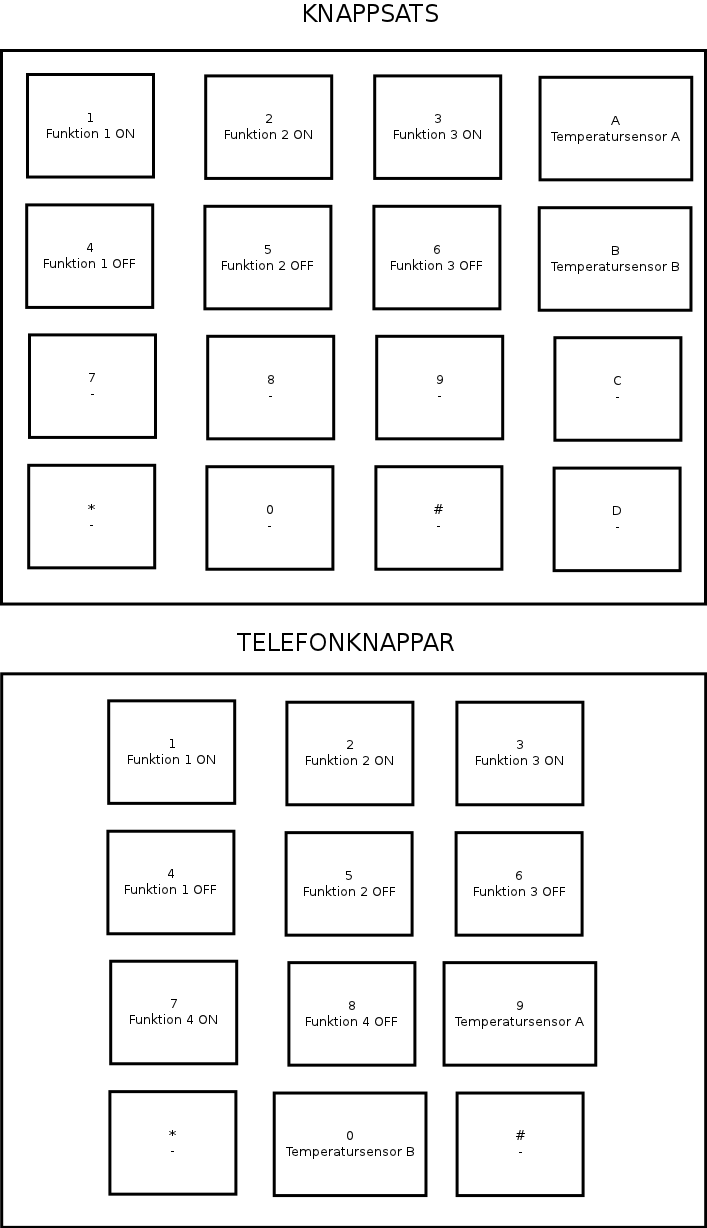
\includegraphics[scale=0.48, angle=0]{UserInterface.png}
			\label{fig:UserInterface}
		  	\caption{Knapplayout, Knappsats resp. Telefon}
		\end{figure}

	\section{Blockschema}
		\begin{figure}[ht!]
		  \centering
		      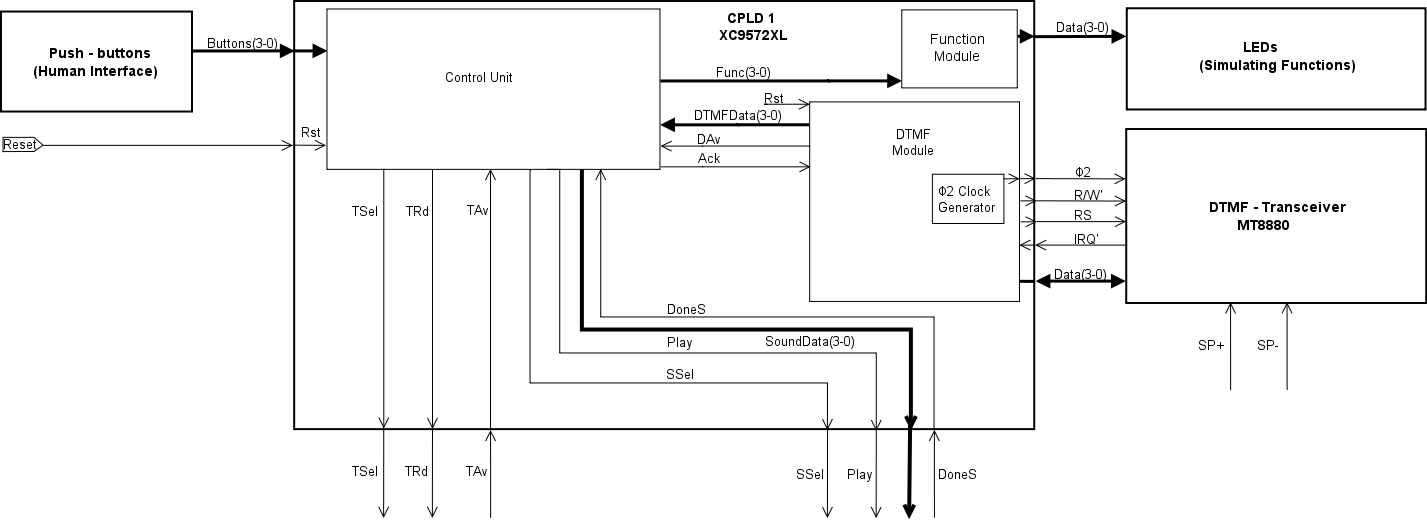
\includegraphics[scale=0.48, angle=90]{BlockDiagramCPLD1.png}
			\label{fig:BlockDiagram1}
		  	\caption{Blockschema (CPLD1)}
		\end{figure}

		\begin{figure}[ht!]
		  \centering
		      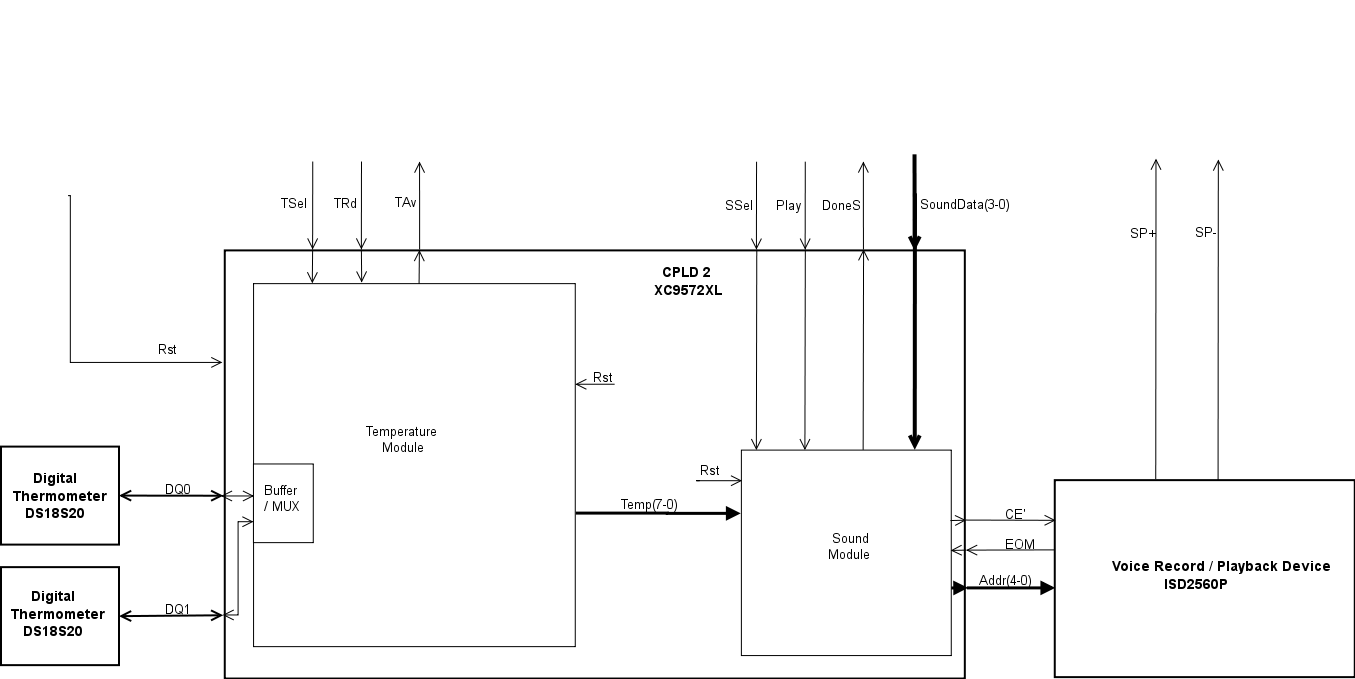
\includegraphics[scale=0.48, angle=90]{BlockDiagramCPLD2.png}
			\label{fig:BlockDiagram2}
		  	\caption{Blockschema (CPLD2)}
		\end{figure}

	\section{Komponentlista}

		\begin{tabular}{ l r}
		   	Matningsspänning & +5V\\
		   	Strömförbrukning & ~80mA\\
		   	Temperaturmätspann & +/- 31.5 C\\
			Temperaturupplösning & 0.5 C\\	
		\end{tabular}

	\section{Kretsschema}

		\begin{figure}[ht!tb]
		  \centering
		      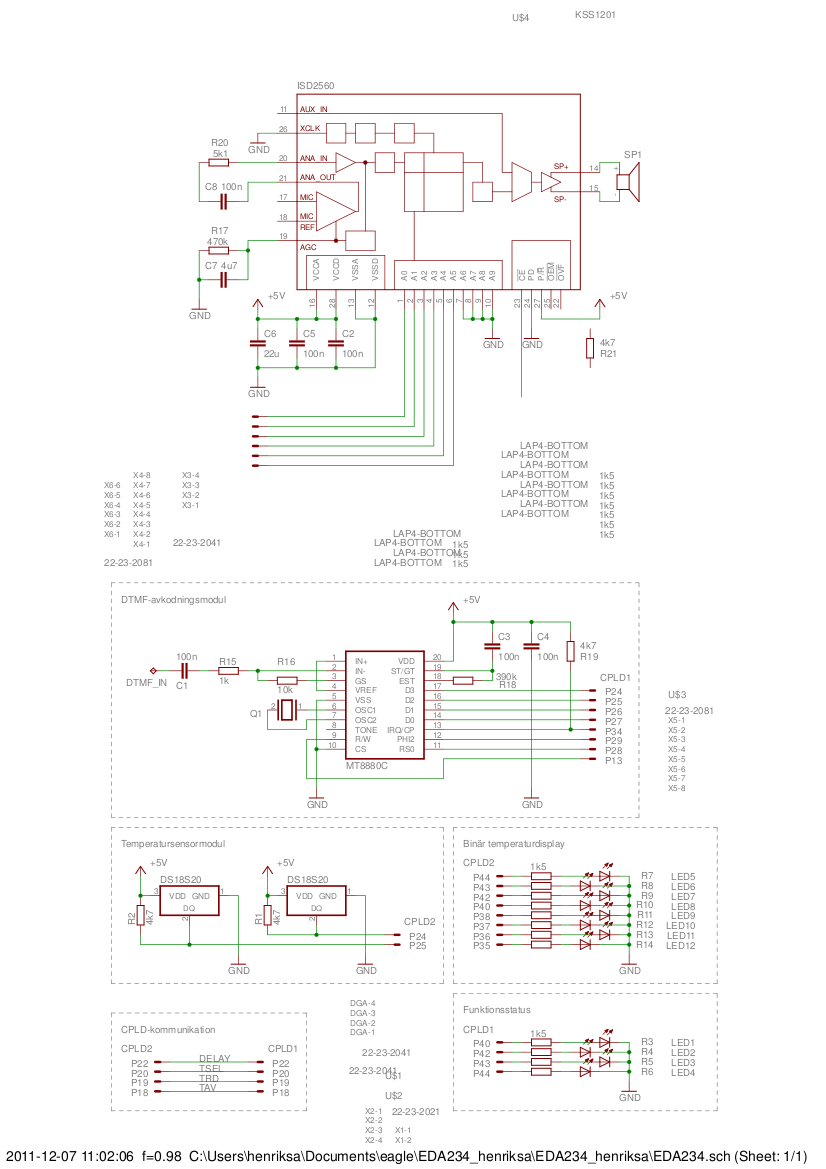
\includegraphics[scale=0.7, angle=0]{schema.png}
			\label{fig:schema}
		  	\caption{Kretsschema}
		\end{figure}

	\section{Kretskortslayout}

	\begin{figure}[ht!]
	  \centering
	      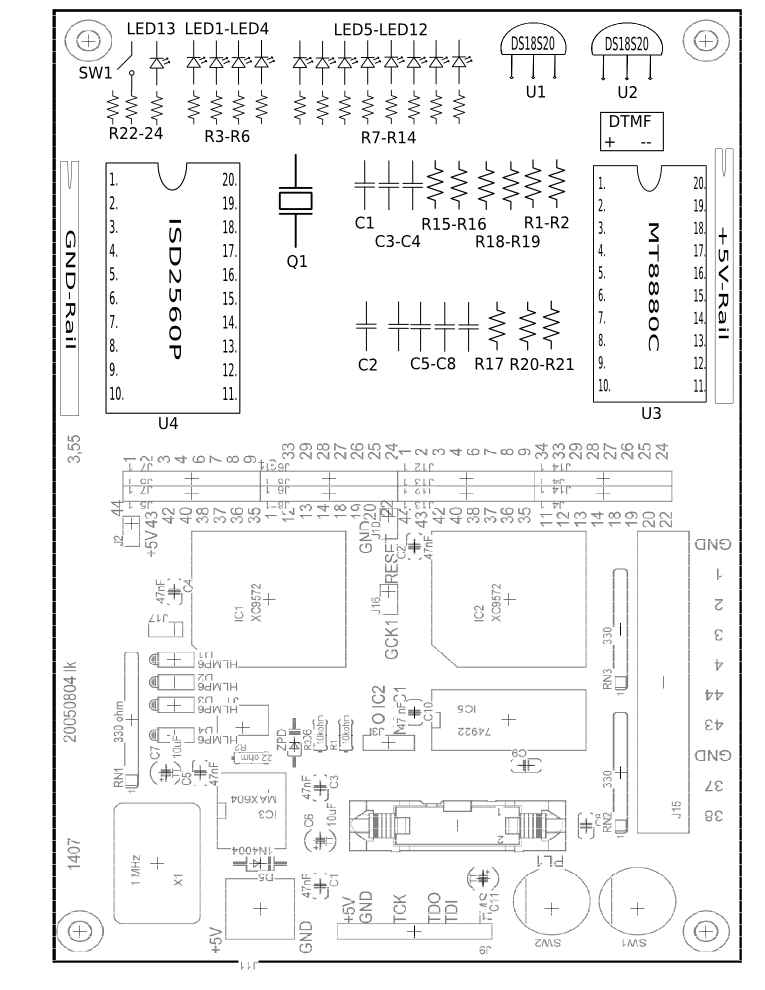
\includegraphics[scale=0.7, angle=0]{layout.png}
		\label{fig:layout}
	  	\caption{Kretskortslayout}
	\end{figure}
	
	\section{Timingdiagram}

		\begin{figure}[ht!tb]
		  \centering
		      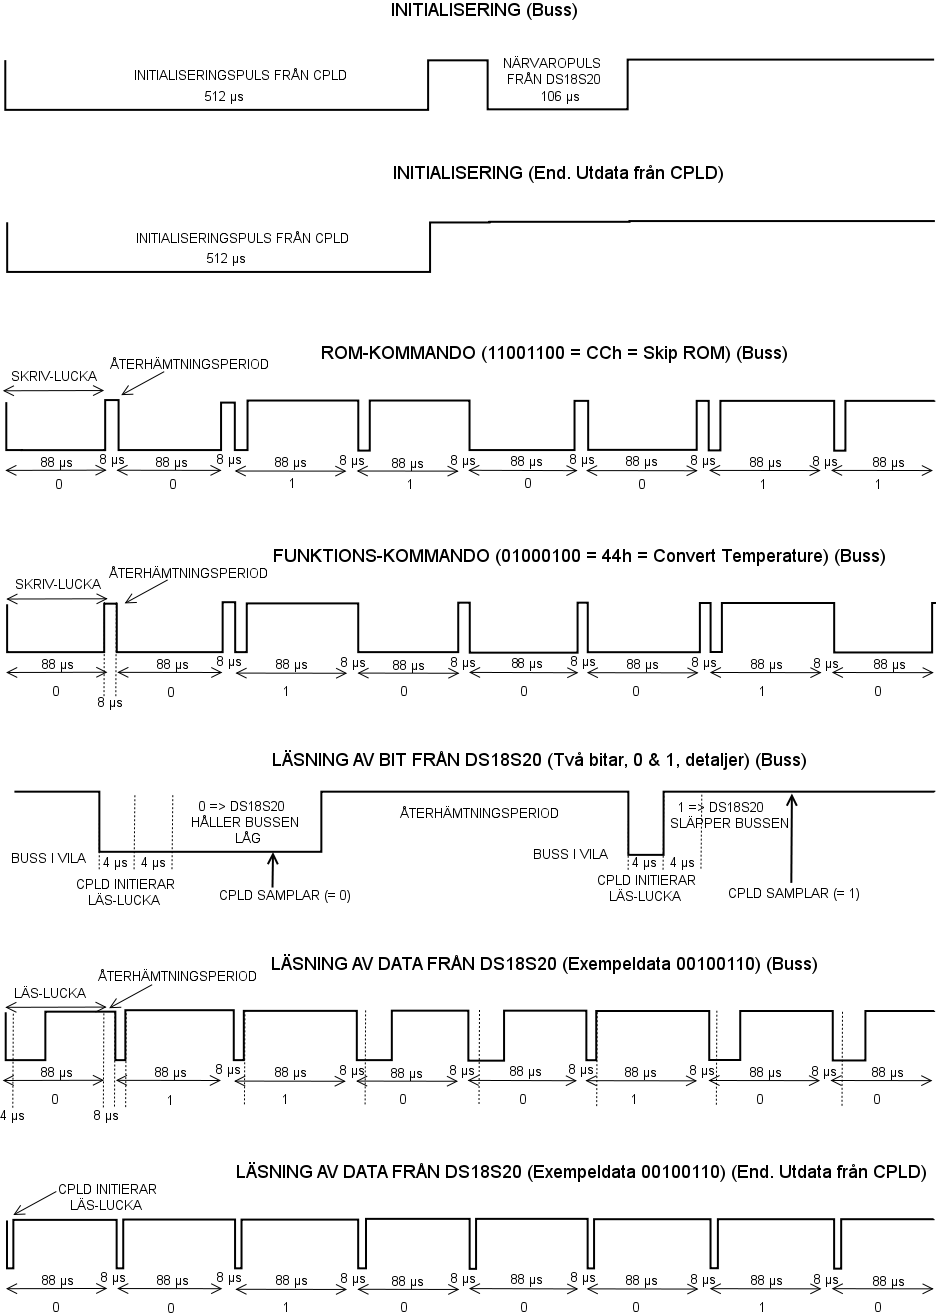
\includegraphics[scale=0.5, angle=0]{TempTiming.png}
			\label{fig:TempTiming}
		  	\caption{Timingdiagram för Temperaturmodulen}
		\end{figure}

	\section{Signallista}
	\begin{tabular}{l c c r}
		\\{\bf Signal} & {\bf Från} & {\bf Till} & {\bf Beskr.}\\ \\
		clk & Extern & Allt & Global Klocksignal\\
		rst & Extern & Allt & Global Resetsignal\\
		Buttons[3..0] & Knappsats & Knappsatsmodul & Indatavektor\\
		KBDav & Knappsats & Knappsatsmodul & Availablesignal\\
		FuncData[3..0] & Funktionsmodul & FunktionsLEDs & Funktionsstyrning\\
		DTMFData[3..0] & DTMF-Modul & MT8880 & Databuss till MT8880 (bidir.)\\
		\(\Phi\)2 & DTMF-Modul & MT8880 & Klocksignal till MT8880\\
		R/W & DTMF-Modul & MT8880 & Read/Write till MT8880\\
		RS0 & DTMF-Modul & MT8880 & Intieringssignal till MT8880\\
		IRQ & MT8880 & DTMF-Modul & Interruptsignal från MT8880\\

		KData[3..0] & Knappsatsmodul & Styrenhet & Data från knappsatsmodul\\
		KAv & Knappsatsmodul & Styrenhet & Availablesignal från knappsatsmodul\\
		KAck & Styrenhet & Knappsatsmodul & Ack. till knappsatsmodul\\

		TSel & Styrenhet & Temperaturmodul & Sensorselectsignal\\
		TRd & Styrenhet & Temperaturmodul & Read-signal (starta läsning)\\
		TAv & Temperaturmodul & Styrenhet & Availablesignal, valid data\\

		SData[3..0] & Styrenhet & Ljudmodul & Ljudadressbuss\\
		SSel & Styrenhet & Ljudmodul & Selectsignal för temperatur/ljud\\
		SPlay & Styrenhet & Ljudmodul & Play-signal (spela ljud)\\
		SDone & Ljudmodul & Styrenhet & Signallerar uppspelning färdig\\

		DData[3..0] & DTMF-Modul & Styrenhet & DTMF-Databuss\\
		DAv & DTMF-Modul & Styrenhet & Availablesignal från DTMF-Modul\\
		DAck & Styrenhet & DTMF-Modul & Acknowledgement från Styrenhet\\

		FData[3..0] & Styrenhet & Funktionsmodul & Funktionsstatusbuss\\

		SP+ & ISD250P & MT8880 & Analog ljudsignal (+)\\
		SP- & ISD250P & MT8880 & Analog ljudsignal (-)\\

		DQ0 & Temperaturmodul & DS18S20 & Seriell 1-trådsbuss (bidir.)\\
		DQ1 & Temperaturmodul & DS18S20 & Seriell 1-trådsbuss (bidir.)\\

		Temp[7..0] & Temperaturmodul & Ljudmodul & Temperaturdatabuss\\

		Addr[4..0] & Ljudmodul & ISD2560P & Adressbuss till ISD2560P\\
		CE & Ljudmodul & ISD2560P & Chip-Enable från ljudmodul\\
		EOM & IDS2560P & Ljudmodul & End-Of-Message från ISD2560P\\\\
	\end{tabular}

	\section{Arbetsfördelning}

	\begin{tabular}{l c r}
		\\{\bf Namn} & {\bf Moduler / Ansvar} & {\bf Övrigt}\\
		Fredrik Brosser 	& ?? 	& ??\\
		Karl Buchka 		& ?? 	& ??\\
		Andreas Henriksson 	& ?? 	& ??\\
		Johan Wolgers 		& ??	& ??\\\\
	\end{tabular}

	\section{Programlistningar}
	\label{sec:programlistningar}	

\end{document}
